\newpage

\section{Versuchsaufbau}
Der allgemeine Versuchsaufbau ist in Abb.1 zu sehen. Die zu untersuchende, würfelförmige
Probe ist mit einer Heizwicklung umgeben und mit einem Pt-100-Widerstand verbunden. Die
Heizwicklung hat die Aufgabe, die Probe zu erwärmen und ist daher an ein Konstantstromgerät
angeschlossen. Der Widerstand ist an einem Ohmmeter angebracht, welches sich außerhalb der
Apparatur befindet. Die Probe hängt in einem Kupfer-Zylinder, welcher die Effekte von
auftretender Wärmestrahlung ausgleicht. Um diesen Zylinder ist wieder eine Heizwicklung
angebracht, die an eine separaten Stromversorgung angeschlossen ist. Zudem ist dort wieder
ein Pt-100-Widerstand angebracht, welcher an ein Ohmmeter angeschlossen ist. Dieser
Kupfer-Zylinder hängt selbst in dem Rezipenten, welcher einen
Zugang zu einer Vakuumpumpe und einer Helium-Gasflasche besitzt. Zwischen Rezipient und
Heliumflasche befindet sich aus Sicherheitsgründen ein Absperhahn und ein Reduzierventil.
Der Rezipient hängt wiederum in einem Dewar-Gefäß, welches mit flüssigem Stickstoff befüllt
wird. Die einzelnen Komponenten hängen jeweils in einander, da so der Energieaustausch durch
Wärmeleitung unterbunden wird. Das spätere Evakuieren schließt zudem den Energieaustausch
durch Konvektion aus.
\begin{figure}[h!]
 \centering
 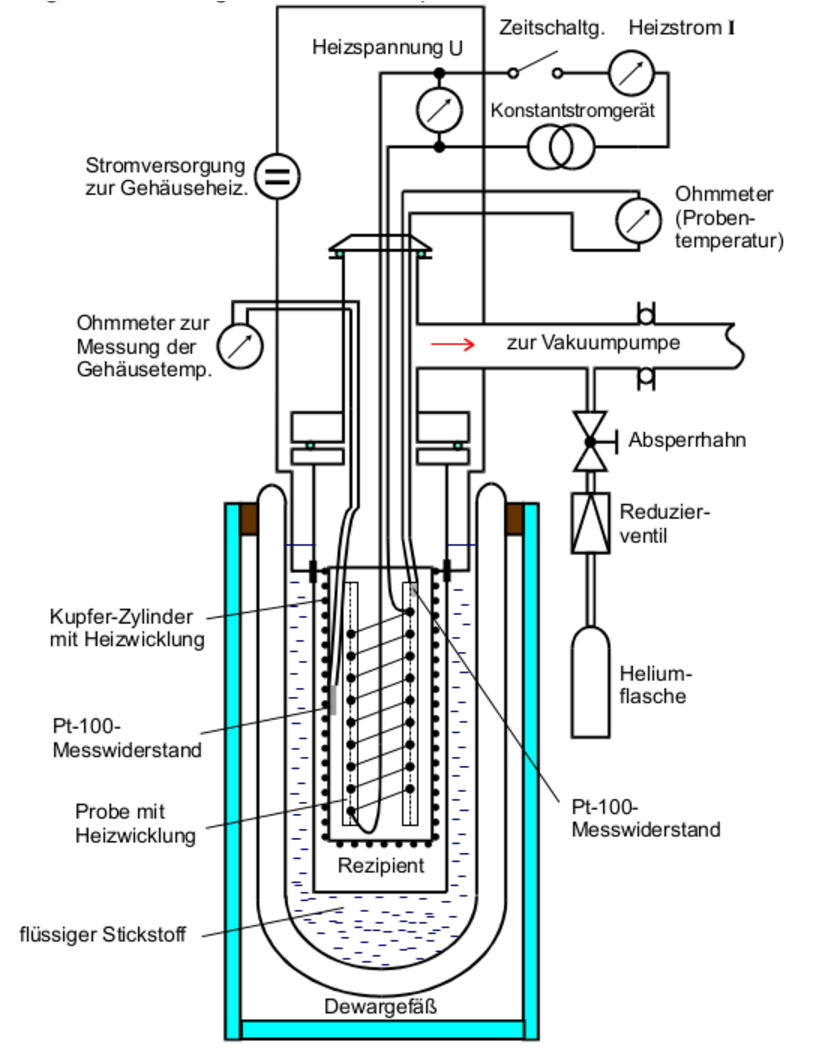
\includegraphics[width=0.6\textwidth]{rohdaten/V47.pdf}
 \caption{Aufbau der Messung zur Bestimmung der Molwärme von Festkörpern. \cite{anleitung}}
 \label{fig:Versuchsaufbau1}
\end{figure}
\FloatBarrier

\section{Durchführung}
\label{sec:Durchführung}
Zu Beginn wird der Rezipient evakuiert und mit gasförmigem Helium befüllt.
Dies hat die Aufgabe, die Wärmeleitung zwischen Rezipient und Kupferzylinder zu optimieren.
Währenddessen wird flüssiger Stickstoff in das Dewar-Gefäß, in dem der Rezipiert
hängt, bis zur Oberkante befüllt. Wenn die Probe auf 80$\,$K abgekühlt ist, wird die Heliumzufuhr
geschlossen und der Rezipient erneut evakuiert. Zudem wird ein
Konstantstrom an der Probe an angelegt. Während der Temperaturunterschied zwischen
Probe und Kupfer-Zylinder bei null gehalten wird, werden beide so beheizt, dass sie in einem
Heizintervall eine Temperaturerhöhung von $\SIrange{7}{10}{\kelvin}$ erfahren. In Abständen von
$\SI{10}{\kelvin}$ werden die Widerstände der Pt-100-Elemente (aus denen die Temperatur errechnet wird),
sowie das zwischenliegende Zeitintervall erfasst. Dies wiederholt sich im Rahmen von $\SIrange{80}{300}{\kelvin}$.
